% **************************************************
% Clean Thesis
% -- A LaTeX Style for Thesis Documents --
%
% Copyright (C) 2011-2014 Ricardo Langner
% **************************************************
%
% Readme:
% ----------------------------------------
% *** Clean, Simple, Elegant ***
% "Clean Thesis" is a LaTeX style for thesis documents, developed
% for my diplom thesis (Diplomarbeit). The style can be understood
% as my personal compromise - a typical clean looking scientific
% document combined and polished with minor beautifications.
%
% The design of this "Clean Thesis" style is inspired
% by user guide documents from Apple Inc.
%
% Note: If you are looking for an exact and correct style regarding
% typographic rules, please have a look at the "Classic Thesis Style"
% (see http://www.miede.de/index.php?page=classicthesis).
%
% *** Donation = Postcard ***
% Based on the idea of Andr\'e Miede: If you like the "Clean Thesis"
% style I would be very pleased about a donation in the form of a
% POSTCARD. You can find my address in the file Clean-Thesis.pdf.
% I am going to collect all postcards and exhibit them at the website
% I mentioned.
%
% *** Idea and Inspiration ***
% The idea of providing my customized style for thesis documents
% passed through my mind while writing my own thesis. Motivated and
% inspired by the superb "Classic Thesis Style"
% (see http://www.miede.de/index.php?page=classicthesis) by Andr\'e Miede
% (thanks to Andr\'e for doing a great job) I decided to collect all
% design and style related functionality in a separate LaTeX style and
% provide this style to other thesis writers.
%
%
% License Information:
% ----------------------------------------
% "Clean Thesis" is free software: you can redistribute it and/or modify
% it under the terms of the GNU General Public License as published by
% the Free Software Foundation, either version 3 of the License, or
% (at your option) any later version.
%
% "Clean Thesis" is distributed in the hope that it will be useful,
% but WITHOUT ANY WARRANTY; without even the implied warranty of
% MERCHANTABILITY or FITNESS FOR A PARTICULAR PURPOSE.  See the
% GNU General Public License for more details.
%
% You should have received a copy of the GNU General Public License
% along with this program.  If not, see <http://www.gnu.org/licenses/>.
% **************************************************


% **************************************************
% Document Class Definition
% **************************************************
\documentclass[%
	paper=A4,					% paper size --> A4 is default in Germany
	twoside=true,				% onesite or twoside printing
	openright,					% doublepage cleaning ends up right side
	parskip=full,				% spacing value / method for paragraphs
	chapterprefix=true,			% prefix for chapter marks
	11pt,						% font size
	headings=normal,			% size of headings
	bibliography=totoc,			% include bib in toc
	listof=totoc,				% include listof entries in toc
	titlepage=on,				% own page for each title page
	captions=tableabove,		% display table captions above the float env
	draft=false,				% value for draft version
]{scrreprt}%

\usepackage{polski}
\usepackage[utf8]{inputenc} % defines file's character encoding
\usepackage[T1]{fontenc} % babel system, adjust the language of the content
\usepackage[polish]{babel}
\usepackage{float}
\usepackage{amsmath}
\usepackage{url}

\pdfinclusioncopyfonts=1
% **************************************************
% Debug LaTeX Information
% **************************************************
%\listfiles

% **************************************************
% Information and Commands for Reuse
% **************************************************
\newcommand{\thesisTitle}{Algorytmy przetwarzania i analizy obrazów trójwymiarowych w zastosowaniach biomedycznych}
\newcommand{\thesisName}{Aleksander Grzyb}
\newcommand{\thesisDate}{2015}

\newcommand{\thesisFirstSupervisor}{dr hab.~inż.~Krzysztof Krawiec}

\newcommand{\thesisUniversity}{\protect{Politechnika Poznańska}}
\newcommand{\thesisUniversityDepartment}{Wydział Informatyki}
\newcommand{\thesisUniversityCity}{Poznań}

% **************************************************
% Load and Configure Packages
% **************************************************

\usepackage[					% clean thesis style
	figuresep=colon,%
	sansserif=false,%
	hangfigurecaption=false,%
	hangsection=true,%
	hangsubsection=true,%
	colorize=full,%
	colortheme=bluemagenta,%
]{cleanthesis}

\definecolor{links}{HTML}{006598}

\hypersetup{					% setup the hyperref-package options
	pdftitle={\thesisTitle},	% 	- title (PDF meta)
	pdfauthor={\thesisName},	% 	- author (PDF meta)
	plainpages=false,			% 	-
	colorlinks=true,			% 	- colorize links?
	linkcolor=links,
	citecolor=links,
	urlcolor=links,
	pdfborder={0 0 0},			% 	-
	breaklinks=true,			% 	- allow line break inside links
	bookmarksnumbered=true,		%
	bookmarksopen=true			%
}

% \raggedbottom

% **************************************************
% Document CONTENT
% **************************************************
\begin{document}

% --------------------------
% rename document parts
% --------------------------
%\renewcaptionname{ngerman}{\figurename}{Abb.}
%\renewcaptionname{ngerman}{\tablename}{Tab.}
\renewcaptionname{polish}{\figurename}{Rys.}
\renewcaptionname{polish}{\tablename}{Tab.}
% \renewcaptionname{english}{\figurename}{Fig.}
% \renewcaptionname{english}{\tablename}{Tab.}

% --------------------------
% Front matter
% --------------------------
\pagestyle{empty}				% no header or footers
% !TEX root = ../thesis-example.tex
%
% ------------------------------------  --> cover title page
\begin{titlepage}
	\pdfbookmark[0]{Cover}{Cover}
	\flushright
	\hfill
	\vfill
	{\LARGE\thesisTitle} \par
	\rule[5pt]{\textwidth}{.4pt} \par
	{\Large\thesisName}
	\vfill
	\textit{\large\thesisDate} \\
\end{titlepage}


% ------------------------------------  --> main title page
\begin{titlepage}
	\pdfbookmark[0]{Titlepage}{Titlepage}
	\tgherosfont
	\centering

	{\Large \thesisUniversity} \\[4mm]
	
\includegraphics[width=12cm]{gfx/logopp} \\[2mm]
	\textsf{\thesisUniversityDepartment} \\

	\vfill
	{\LARGE \color{ctcolormain}\textbf{\thesisTitle} \\[10mm]}
	{\Large \thesisName} \\

	\vfill
	\hspace*{15pt}

	\begin{minipage}[t]{.27\textwidth}
		\raggedleft
		\textit{Promotor}
	\end{minipage}
	\hspace*{10pt}
	\begin{minipage}[t]{.65\textwidth}
		\thesisFirstSupervisor
	\end{minipage} \\[10mm]

	\thesisDate \\

\end{titlepage}


% ------------------------------------  --> lower title back for single page layout
\hfill
\vfill
{
	\small
	\textbf{\thesisName} \\
	\textit{\thesisTitle} \\
	\thesisDate \\
	Promotor: \thesisFirstSupervisor \\
	\textbf{\thesisUniversity} \\
	\thesisUniversityDepartment \\
	\thesisUniversityCity \\
}
		% INCLUDE: all titlepages
\cleardoublepage

\pagestyle{plain}				% display just page numbers

\setcounter{tocdepth}{2}		% define depth of toc
\tableofcontents				% display table of contents\tabularnewline
\cleardoublepage

% --------------------------
% Body matter
% --------------------------
\pagenumbering{arabic}			% arabic page numbering
\setcounter{page}{1}			% set page counter
\pagestyle{maincontentstyle} 	% fancy header and footer

% !TEX root = ../thesis.tex
%
\chapter{Wstęp}
\label{sec:wstep}

Gwałtowny rozwój technologii w ostatnim wieku ma ogromny wpływ na metody diagnostyczne w medycynie. Dzięki nowym technologiom takim jak optyczna tomografia koherencyjna (ang. \textit{optical coherence tomography, OCT}, sekcja \ref{sec:obrazowanie_oct}) lekarze są w stanie zastąpić inwazyjne metody diagnostyczne, których przeprowadzenie stanowi ryzyko dla zdrowia pacjenta. Postęp w dziedzinie informatyki, a w szczególności algorytmów przetwarzania obrazów przyczynia się do wzrostu jakości obrazów diagnostycznych przez co lekarze są w stanie rozpoznać choroby skuteczniej oraz szybciej.

\section{Opis problemu}
\label{sec:wstep:opis_problemu}

Jednym z najbardziej popularnych zastosowań optycznej tomografii koherencyjnej jest badanie siatkówki oka. Wykorzystanie OCT pozwala zastąpić inwazyjną metodę diagnozy siatkówki polegającej na wstrzyknięciu środka kontrastowego do krwiobiegu pacjenta, a następnie wykorzystaniu jednej z metod obrazowania opierającej się na promieniach rentgenowskich. Użycie środka kontrastowego wiąże się z ryzykiem szkodliwych powikłań na zdrowiu pacjenta tj. reakcje alergiczne, czy bóle głowy. Optyczna tomografia koherencyjna dzięki swojej nieinwazyjnej charakterystyce w badaniu siatkówki jest mocno rozwijana przez wiele ośrodków laboratoryjnych na całym świecie (jednym z przedsięwzięć zajmujących się doskonaleniem OCT jest projekt RIMO-BIOL opisany dokładnie w sekcji \ref{sec:wstep:rimo-biol}, w którego skład wchodzi niniejsza praca). Wynikiem przeprowadzenia optycznej tomografii koherencyjnej są trójwymiarowe obrazy oddające strukturę siatkówki oka (prawy obraz na rysunku \ref{fig:obrazowanie_oct:scan}). Na podstawie trójwymiarowych obrazów są tworzone angiograficzne obrazy \textit{en face} przedstawiające przebieg naczyń krwionośnych (rysunek \ref{sec:obrazowanie_oct:angiografia_oct}). Każdy obraz angiograficzny przedstawia fragment siatkówki oka.

\textbf{Celem niniejszej pracy} jest zaimplementowanie algorytmu, który poprzez pobranie angiograficznych obrazów siatkówki oka wraz z informacją o ich wzajemnych relacjach przestrzennych ma za zadanie automatycznie stworzyć jednolitą mozaikę przedstawiającą całość siatkówki oka. Potrzeba na stworzenie autorskiego algorytmu powstała ze względu na to, że dostępne metody tworzenia mozaiki (ang. \textit{mosaic stitching}) nie dają zadowalających rezultatów ze względu na charakterystykę angiograficznych obrazów OCT.

\subsection{Projekt RIMO-BIOL}
\label{sec:wstep:rimo-biol}

\textbf{Projekt RIMO-BIOL} po tytułem ,,Rozwój interferometrycznych metod optycznych do badania dynamiki układów biologicznych'', w którego skład wchodzi niniejsza praca skupia się na rozwoju mikroskopowych metod optycznych w celu badania dynamiki układów biologicznych. Projekt jest przeprowadzany przez konsorcjum składające się z m. in. Uniwersytetu Mikołaja Kopernika w Toruniu i Politechniki Poznańskiej w Poznaniu. Praca jest finansowana przez Narodowe Centrum Badań i Rozwoju w ramach pierwszej edycji konkursu ,,Program Badań Stosowanych''.

RIMO-BIOL pracuje obecnie nad rozwojem optycznej tomografii koherencyjnej oraz sprzętu jej wykonującej. Wszystkie obrazy wykorzystywane w niniejszej pracy pochodzą z aparatury OCT zbudowanej w ramach projektu. Stworzona technologia w ramach RIMO-BIOL testowana jest w  badaniach:

\begin{enumerate}
\item Siatkówki oka ludzkiego w celu diagnozy cukrzycy na podstawie struktur mikronaczyń w siatkówce oka.
\item Mózgu myszy w celu analizy przebiegu udaru mózgu na podstawie oceny morfologii i przepływu krwi w sieci mikronaczyniowej mózgu.
\item Komórek jajowych na podstawie pomiaru ruchu cytoplazmy.
\end{enumerate}

\subsection{Cele szczegółowe}
\label{sec:wstep:cele_szczegolowe}

Wynikiem niniejszej pracy ma być oprogramowanie realizujące cel niniejszej pracy opisany w \ref{sec:wstep:opis_problemu}, natomiast do celów szczegółowych można zaliczyć:

\begin{enumerate}
\item Rozpoznanie możliwości bibliotek przetwarzania i analizy obrazów w zakresie korejestracji przestrzennej.
\item Wybór bibliotek i środowiska deweloperskiego.
\item Projekt, implementacja i przetestowanie algorytmów przetwarzania obrazów realizujących cel niniejszej pracy.
\item Stworzenie w pełni funkcjonalnego oraz prostego w użyciu programu komputerowego o nazwie \texttt{mostitch}.
\item Przygotowanie dokumentacji technicznej oprogramowania.
\end{enumerate}

\section{Organizacja pracy}
\label{sec:wstep:organizacja_pracy}

Praca zaczyna się od przedstawienia w rozdziale \ref{sec:obrazowanie_oct} technologii optycznej tomografii komputerowej oraz wyjaśnienia zasady jej działania. Następnie w rozdziale \ref{sec:algorytmy_korejestracji} opisano dostępne metody oraz poszczególne kroki niezbędne do stworzenia mozaiki (ang. \textit{mosaic stitching}) w kontekście angiograficznych obrazów OCT. Kolejno w rozdziale \ref{sec:proponowane_algorytmy} szczegółowo opisano zasadę działania wybranych oraz autorskich algorytmów realizujących cel niniejszej pracy. W rozdziale \ref{sec:oprogramowanie:oprogramowanie} zaprezentowano stworzone oprogramowanie, zasadę jego użycia oraz wykorzystane biblioteki. W rozdziale \ref{sec:wyniki_eksperymentow} przedstawiono wynikowe mozaiki powstałe z przykładowych angiograficznych obrazów OCT. Na koniec w rozdziale \ref{sec:podsumowanie_i_wnioski} opisano trudności napotkane podczas pracy oraz możliwy rozwój oprogramowania w przyszłości.



% !TEX root = ../thesis.tex
%
\chapter{Obrazowanie OCT}
\label{sec:obrazowanie_oct}

% Wstęp do OCT

\textbf{Optyczna tomografia koherencyjna} (ang. \textit{optical coherence tomography, OCT}) jest metodą umożliwiającą nieinwazyjne oraz \textit{in vivo} przechwycenie obrazu wnętrza tkanki biologicznej. Zasada działania OCT opiera się na wykorzystaniu fal świetlnych. Dzięki temu rozdzielczość obrazów jest o wiele wyższa niż w ultrasonografii (wykorzystanie fal dźwiękowych), czy rezonansie magnetycznym (wykorzystanie pola magnetycznego). Następnym powodem dużej popularności OCT w medycynie jest bezkontaktowe badanie pacjenta oraz brak wymogu przygotowania pacjenta przed badaniem.

W projekcie RIMO-BIOL (sekcja \ref{sec:wstep:rimo-biol}) OCT wykorzystano do uzyskania szczegółowych obrazów naczyń krwionośnych siatkówki oka. Rysunek \ref{fig:obrazowanie_oct:bscan_vessels} przedstawia przykładowe obrazy siatkówki oka uzyskane poprzez wykorzystanie OCT. Jednym z tych przykładowych obrazów jest angiografia siatkówki oka, która jest obrazem wejściowym do algorytmów omawianych w niniejszej pracy. Sposób powstania angiografii z danych OCT jest wyjaśniony w sekcji \ref{sec:obrazowanie_oct:angiografia_oct}, natomiast ogólna zasada działania OCT jest wyjaśniona w sekcji \ref{sec:obrazowanie_oct:metoda_oct}. Na koniec rozdziału w sekcji \ref{sec:obrazowanie_oct:zastosowania_oct} opisano zastosowania OCT.

\begin{figure}[htb]
	\centering
	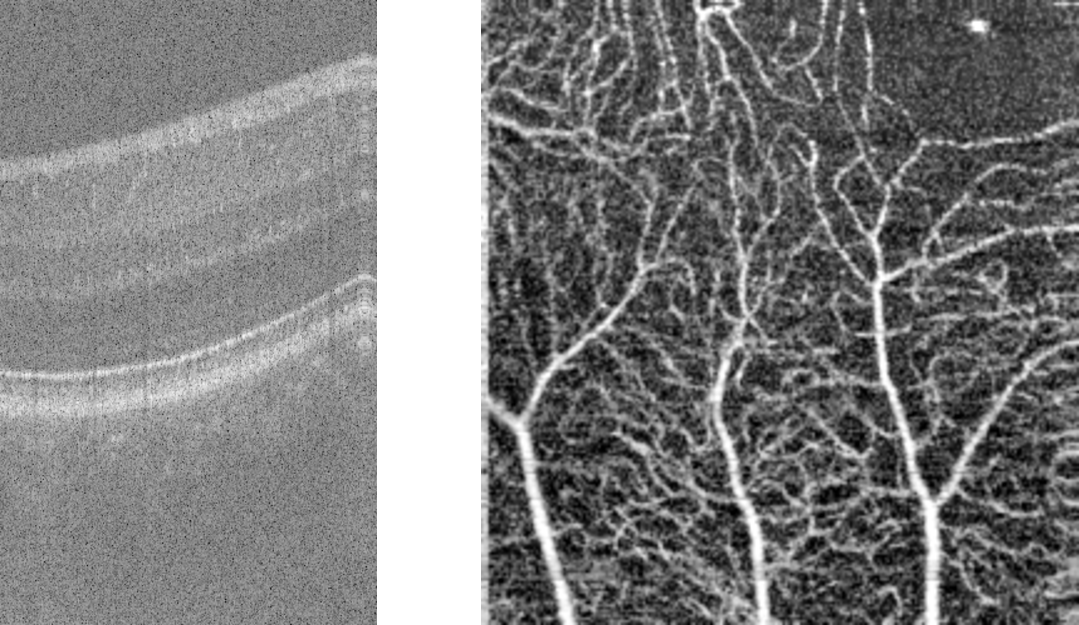
\includegraphics[width=\textwidth]{gfx/bscan_vessels}
	\caption{\textbf{Lewy obraz:} Dwuwymiarowy przekrój siatkówki oka (B-skan). Obraz został uzyskany poprzez połączenie jednowymiarowych A-skanów, które zawierają informację o strukturze tkanki w głąb siatkówki oka. \textbf{Prawy obraz:} Angiografia siatkówki oka uzyskana poprzez przetworzenie danych z OCT.}
	\label{fig:obrazowanie_oct:bscan_vessels}
\end{figure}

% Wyjaśnia zasadę działania OCT, bez wchodzenia w duże teoretyczne detale

\section{Zasada działania OCT}
\label{sec:obrazowanie_oct:metoda_oct}

Optyczna tomografia koherencyjna przechwytuje obrazy wnętrza tkanki poprzez wykorzystanie fal świetlnych. OCT za pomocą generatora wytwarza falę świetlną, która jest skierowana na tkankę pacjenta. Następnie po odbiciu fali poprzez tkankę wiązka jest przechwycona przez detektor. Jedną z dostępnych metod, która umożliwiłaby zlokalizowanie miejsca odbicia fali byłoby zmierzenie czasu pomiędzy wygenerowaniem fali, a zarejestrowaniem jej przez detektor (mechanizm stosowany np. w ultrasonografii z wykorzystaniem fal dźwiękowych), natomiast prędkość światła (\(3\times10^8 \frac{m}{s}\)) wyklucza zastosowanie tego mechanizmu. Zjawisko, które umożliwia dokładne zlokalizowanie miejsca odbicia to \textbf{interferencja światła o niskiej spójności}.

\begin{figure}[htb]
	\centering
	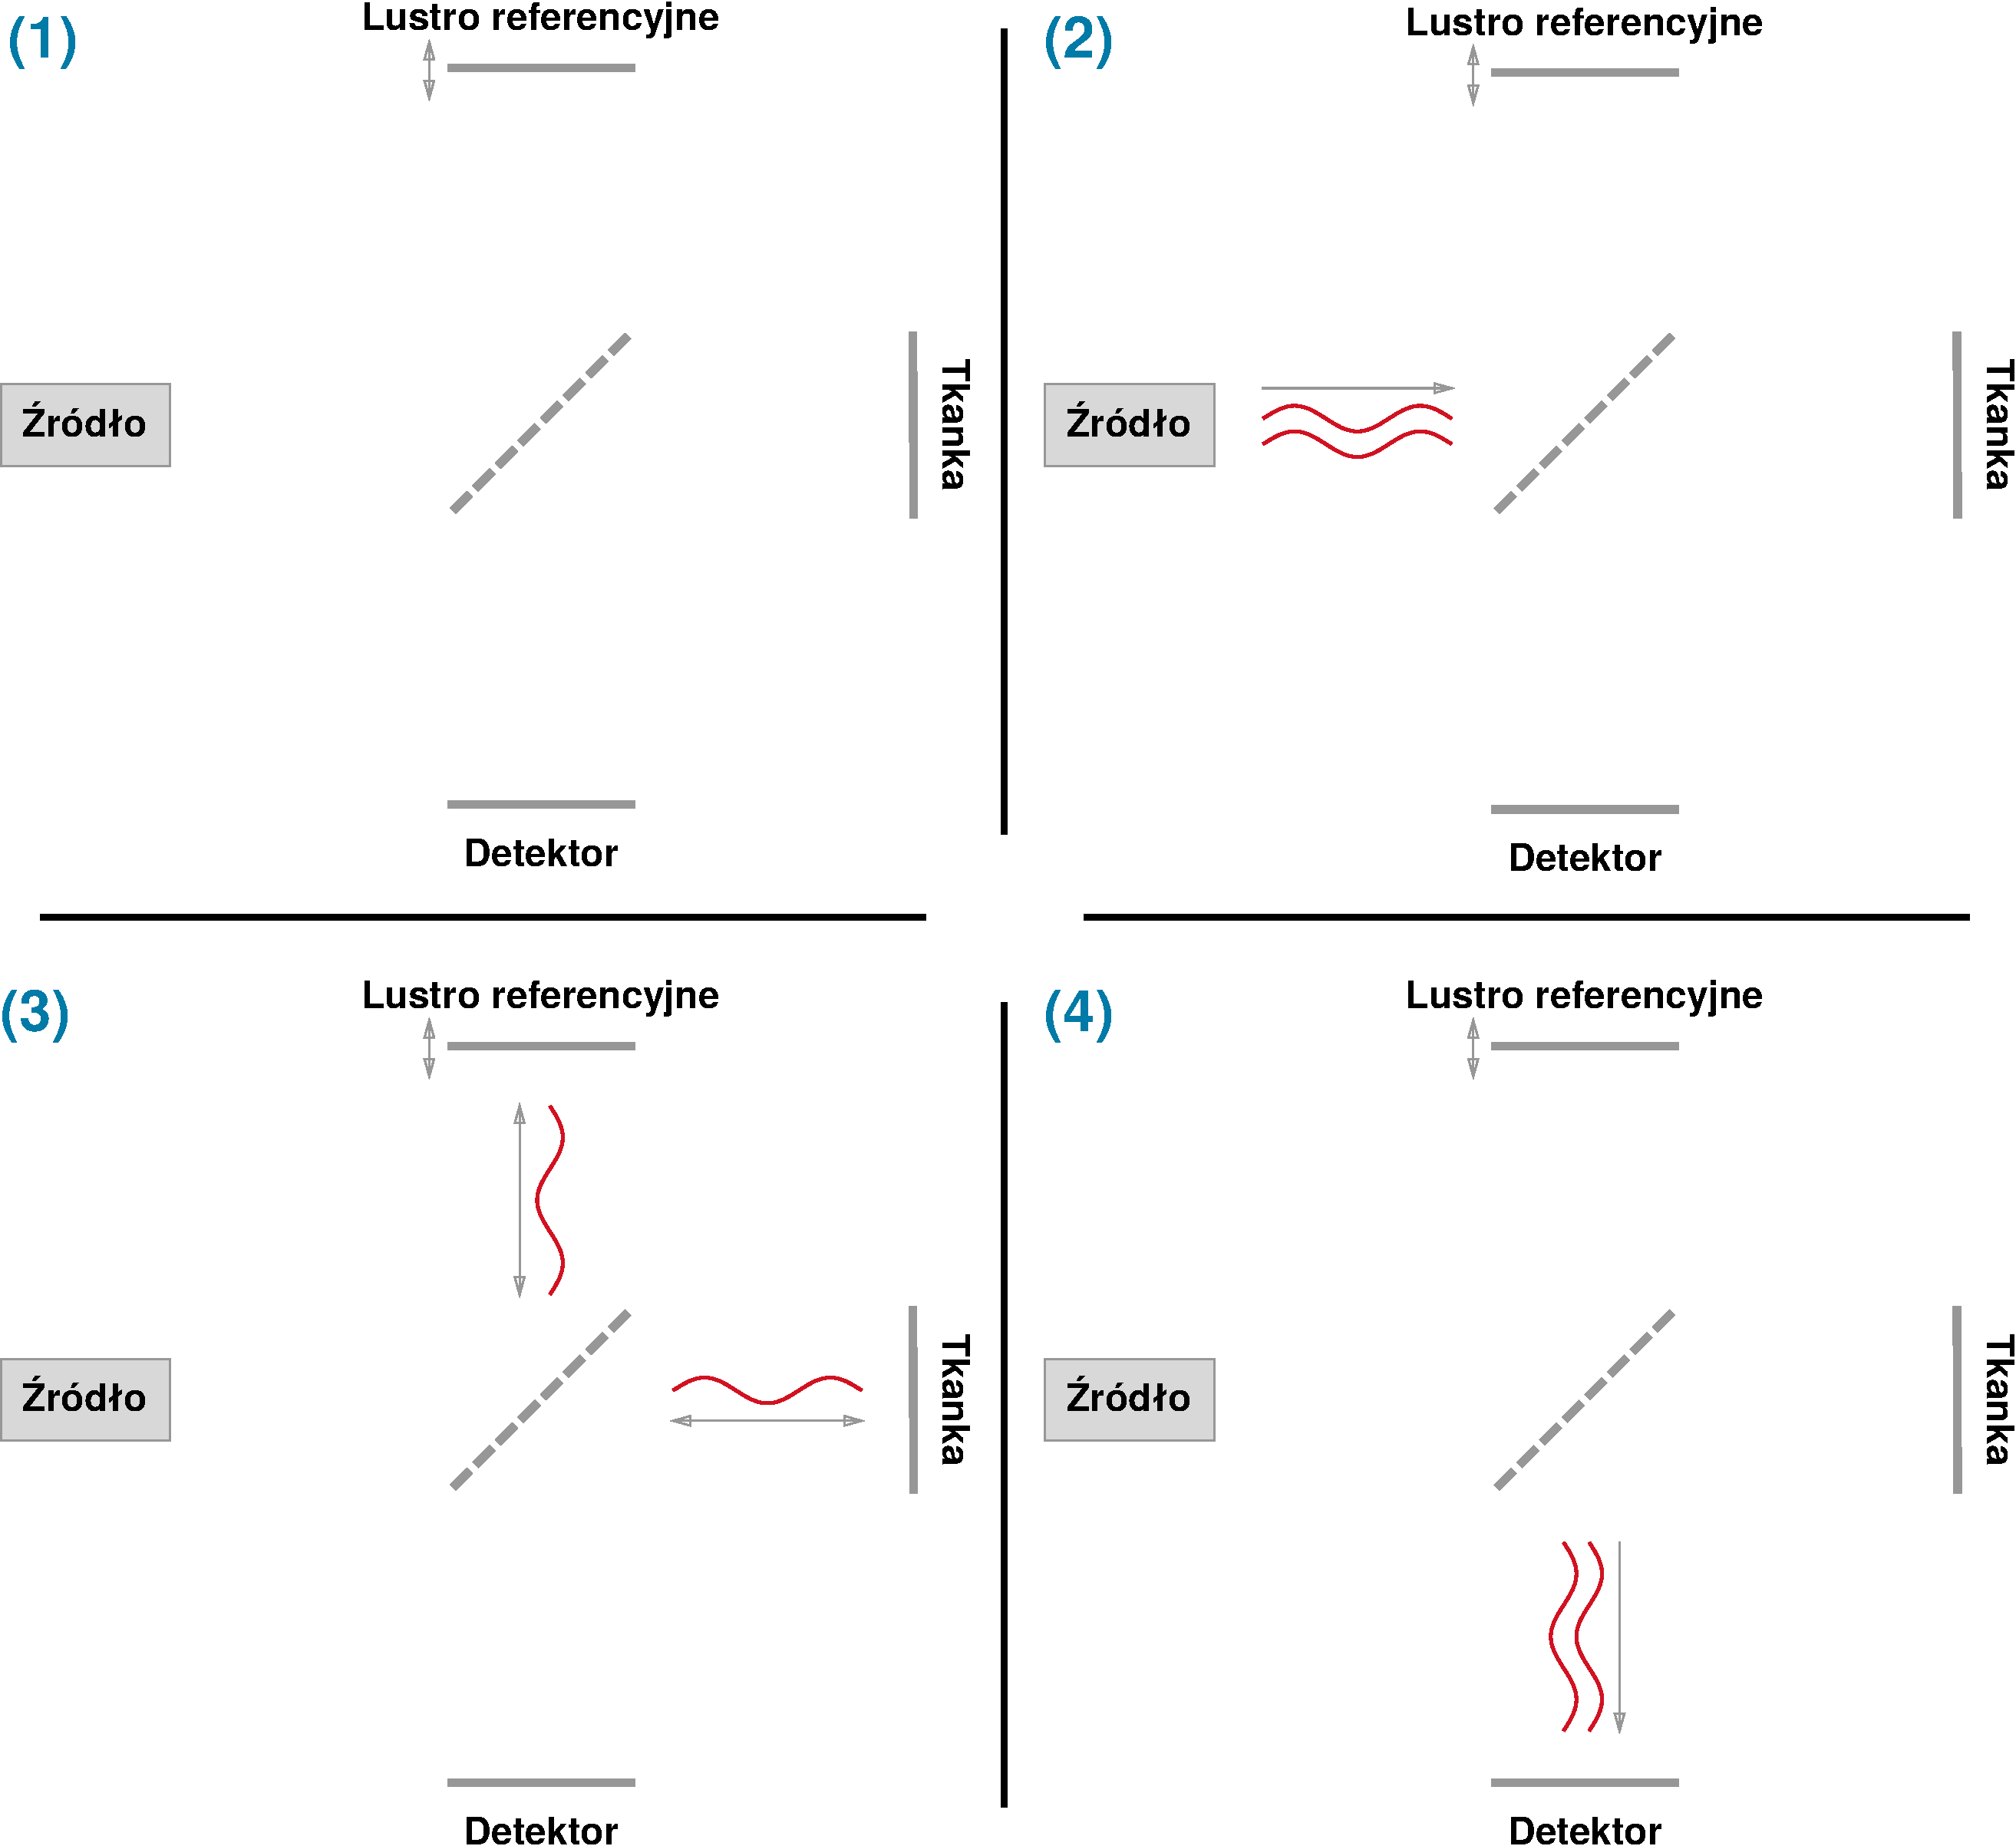
\includegraphics[width=\textwidth]{gfx/oct_phases}
	\caption{Kolejne etapy działania metody OCT. \textbf{(1)} - Etap początkowy. \textbf{(2)} - Źródło wyemitowało wiązkę światła. \textbf{(3)} - Fala rozdzieliła się za pomocą interferometru na wiązkę referencyjną (skierowaną na lustro referencyjne) oraz na wiązkę próbki (skierowaną na tkankę). \textbf{(4)} - Wiązki po odbiciu od lustra referencyjnego i tkanki ponownie łączą się za pomocą interferometru. W tej części występuje zjawisko interferencji, które jest zarejestrowane przez detektor.}
	\label{fig:obrazowanie_oct:oct_phases}
\end{figure}

Rysunek \ref{fig:obrazowanie_oct:oct_phases} składa się z bardzo uproszczonych schematów OCT obrazujących kolejne etapy działania metody. Schematy na rysunku \ref{fig:obrazowanie_oct:oct_phases} składają się z pięciu elementów:

\begin{itemize}

\item \textbf{Źródła} - Źródło (np. dioda superluminescencyjna) światła podczerwonego będąca falą o niskiej spójności.
\item \textbf{Rozdzielacza wiązek} (na rysunku \ref{fig:obrazowanie_oct:oct_phases} przedstawiony za pomocą przerywanych linii na środku każdego schematu) - Interferometr (np. Michelsona) umożliwiający rozdzielenie fali na dwie wiązki oraz następne ich połączenie.
\item \textbf{Lustro referencyjne} - Lustro, które odbija wiązkę referencyjną. Posiada możliwość oddalania oraz przybliżania się względem interferometru.
\item \textbf{Tkanka} - Badana tkanka odbijająca wiązkę próbki.
\item \textbf{Detektor} - Rejestruje zjawisko interferencji związek.

\end{itemize}

Najbardziej istotnym etapem wymaganym do zrozumienia mechanizmu OCT jest etap (4) pokazany na rysunku \ref{fig:obrazowanie_oct:oct_phases}. W tym kroku wiązka referencyjna i wiązka próbki łączą się i zachodzi zjawisko interferencji. Dzięki temu, że wiązki są falami o niskiej spójności interferencja zachodzi tylko na małej długości zwanej \textit{coherence length}. Odkrywając za pomocą detektora charakterystyczny wzorzec interferencji występujący na \textit{coherence length} OCT w stanie precyzyjnie odczytać informację odnośnie struktury wnętrza tkanki. Badanie warstw tkanki o różnej głębokości przedstawia rysunek \ref{fig:obrazowanie_oct:tissue_layers}.

\begin{figure}[htb]
	\centering
	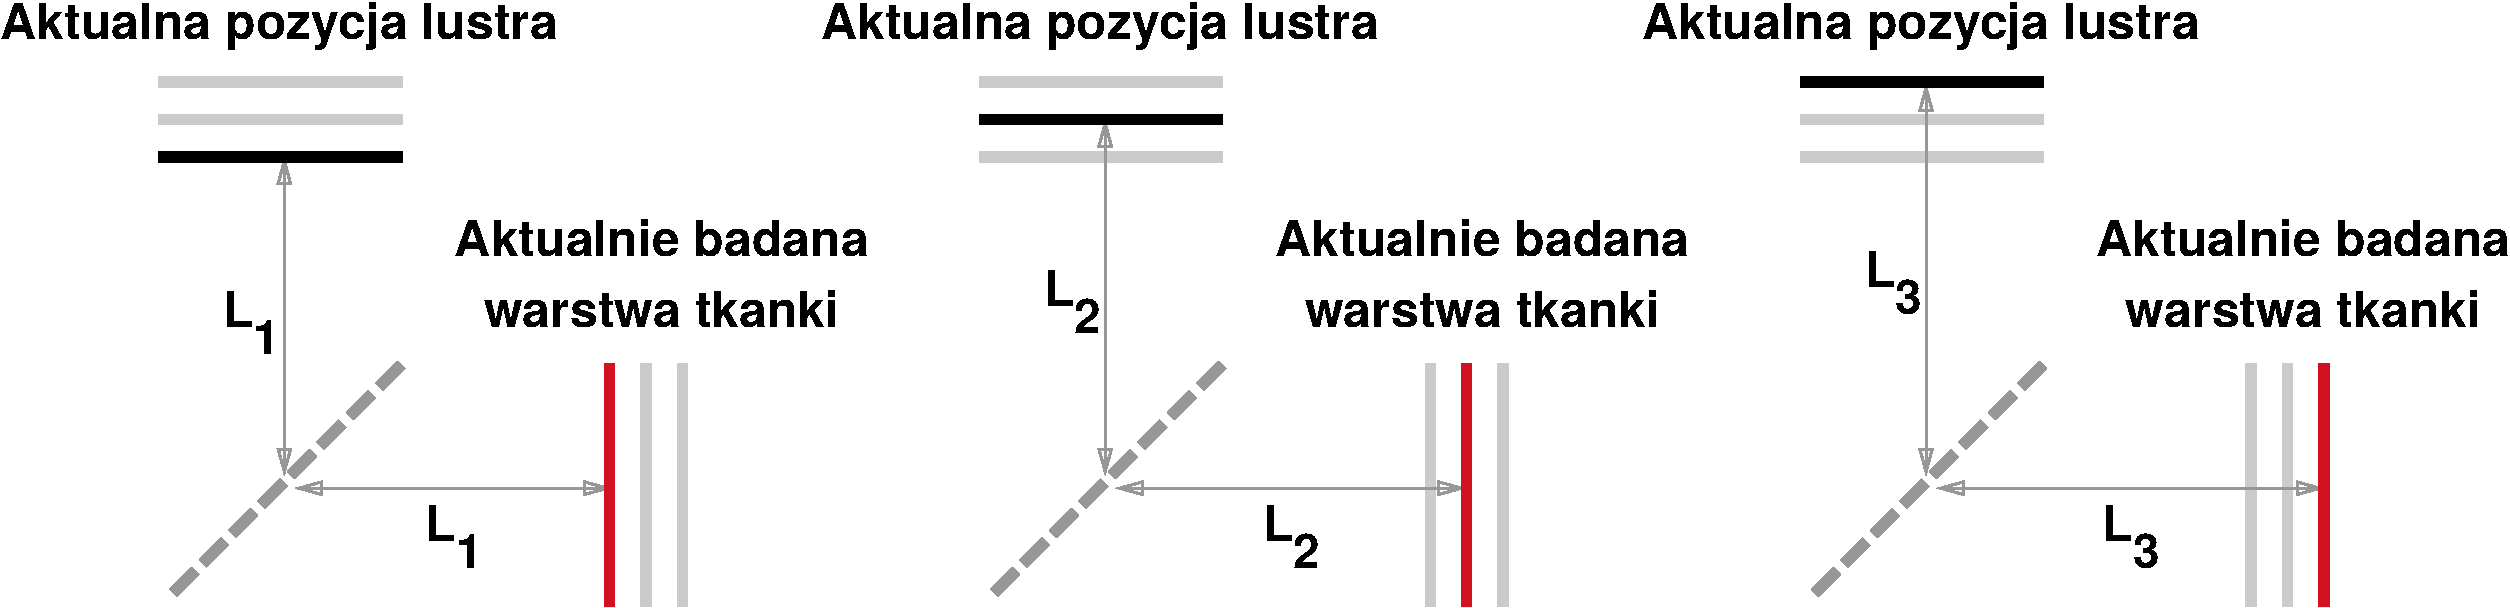
\includegraphics[width=\textwidth]{gfx/tissue_layers}
	\caption{Kolejne etapy badania głębszych warstw tkanki dzięki przesuwaniu lustra referencyjnego. Aktualna pozycja lustra referencyjnego jest zaznaczona kolorem czarnym, natomiast aktualnie badana warstwa tkanki jest zaznaczona kolorem czerwonym.}
	\label{fig:obrazowanie_oct:tissue_layers}
\end{figure}

\subsection{Metoda uzyskania trójwymiarowego obrazu tkanki}

Poprzez poruszenie lustra referencyjnego pomiary przeprowadzane są w głąb tkanki (wzdłuż osi Z). Zbiór pomiarów w głąb tkanki nazywa się A-skanem (obraz jednowymiarowy). Powtarzając ten proces w osi X lub Y i następnie poprzez połączenie sąsiadujących A-skanów otrzymuje się przekrój tkanki zwany B-skanem (obraz dwuwymiarowy). Proces uzyskania B-skanów można powtórzyć dla sąsiadujących przekrojów. Poprzez połączenie otrzymanych B-skanów otrzymuje się trójwymiarowy obraz tkanki. Na rysunku \ref{fig:obrazowanie_oct:scan} \cite{Kraus:12} przedstawione są poszczególne skany.

\begin{figure}[htb]
	\centering
	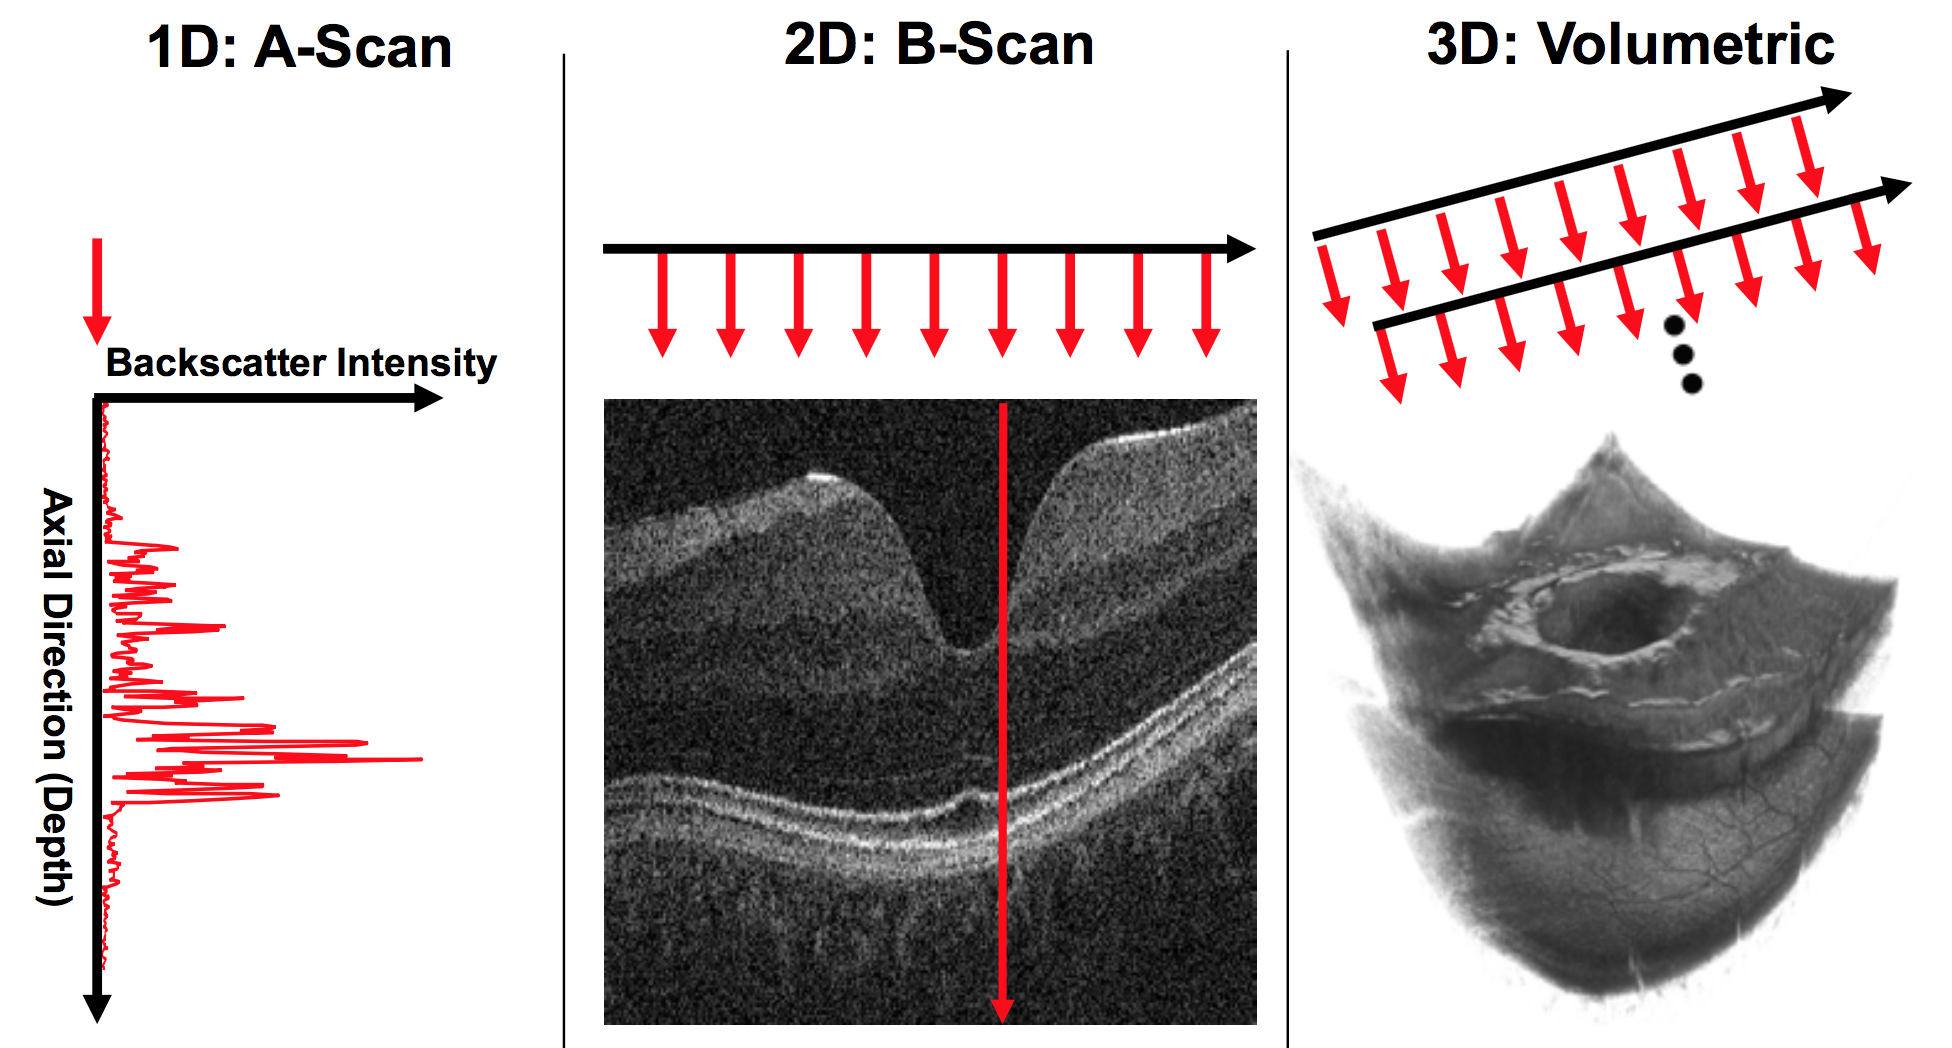
\includegraphics[width=\textwidth]{gfx/scans}
	\caption{\cite{Kraus:12} \textbf{Lewy obraz:} Pojedynczy A-skan wykonany w głąb tkanki. \textbf{Środkowy obraz:} Otrzymany B-skan poprzez połączenie A-skanów. \textbf{Prawy obraz:} Trójwymiarowy obraz tkanki stworzony poprzez połączenie B-skanów.}
	\label{fig:obrazowanie_oct:scan}
\end{figure}

\subsection{OCT w domenie częstotliwości}

Metoda OCT wykonująca ruchy lustrem referencyjnym jest zwana metodą OCT w domenie czasu (ang. \textit{time-domain OCT, TdOCT}). Alternatywną oraz nowszą metodą od TdOCT jest OCT w domenie częstotliwości (ang. \textit{Fourier-domain OCT, FdOCT}). FdOCT umożliwia 100 razy szybsze \cite{Strong:11} skanowanie w porównaniu do TdOCT. TdOCT jest w stanie wykonać ok. 400 A-skanów w przeciągu sekundy, natomiast FdOCT jest ich w stanie wykonać dziesiątki tysięcy. Szybsze skanowanie poprawia również jakość skanów ze względu na to, że pacjent ma mniejszą szansę poruszenia okiem podczas skanowania (ruch oka w trakcie skanowania przyczynia się do powstania artefaktów ruchu na obrazach OCT). Oprócz poprawy szybkości skanowania FdOCT ma wyższą rozdzielczość w przedziale od 3 do 7 mikrometrów \cite{Strong:11}. Jest to poprawa względem TdOCT o 8-10 mikrometrów.

Większa szybkość oraz rozdzielczość FdOCT w porównaniu do TdOCT jest możliwa dzięki dwóm modyfikacjom technicznym:

\begin{enumerate}

\item FdOCT jako źródło światła wykorzystuje laser o wysokiej szerokości pasma, co znacząco zwiększa rozdzielczość.
\item FdOCT jako detektor wykorzystuje spektrometr, który przeprowadza analizę widma fali (połączona wiązka referencyjna i próbki), która dotarła do spektrometru z interferometru. Transformata Fouriera na widmie fali tworzy A-skan tkanki. Dzięki tej technice FdOCT wyeliminowało potrzebę ruszania lustrem referencyjnym co znacząco zwiększa szybkość skanowania.

\end{enumerate}

FdOCT posiada również wady. Pierwszą z nich jest cena. TdOCT jest droższy ze względu na wykorzystanie drogiego lasera jako źródła światła przez co jest wykorzystywany tylko w celach badawczych. Druga wada wynika z szybkości powstawania A-skanów. Szybsze skanowanie prowadzi do utraty jakości obrazów (zastosowanie techniki przetwarzania sygnałów zwanej \textit{oversampling} może zrekompensować tę stratę).

% Wyjaśnia zasadę powstawania obrazów angiograficznych z danych OCT

\section{Angiografia OCT}
\label{sec:obrazowanie_oct:angiografia_oct}

Angiografia to technika służąca do wizualizacji naczyń krwionośnych i organów ciała. W większości przypadków w medycynie angiografia jest wykonywana poprzez wstrzyknięcie pacjentowi środka kontrastowego, który nie przepuszcza promieni rentgenowskich. Następie by stworzyć obrazy angiograficzne wykorzystuje się jedną z technik obrazowania (np. fluoroskopię) opartą o promienie rentgenowskie. Metoda oparta na stosowaniu środka kontrastowego ma jedną znaczącą wadę, jako technika inwazyjna może prowadzić do reakcji alergicznych na środek kontrastowy oraz jest przeciwwskazana kobietom w ciąży i dzieciom. Z tego powodu nieustannie poszukiwane są metody, które jednocześnie są nieinwazyjne i tworzą obrazy o jakości porównywalnej do metod inwazyjnych.

Angiografia OCT poprzez wykorzystanie A-skanów i B-skanów OCT jest w stanie stworzyć obraz \textit{en face} naczyń krwionośnych siatkówki oka. Przykład takiego obrazu znajduje się na rysunku \ref{sec:obrazowanie_oct:angiografia_oct}.

\subsection{Sposób powstania obrazu angiograficznego}

Obrazy angiograficznie użyte w niniejszej pracy powstały za pomocą metody zwanej \textit{Speckle Variance Detection} polegającej na liczeniu wariancji dla każdego piksela pomiędzy sąsiadującymi B-skanami. Wartość wariancji w obszarach gdzie występuje przepływ krwi (naczynia krwionośne) jest wyższa od obszarów, w których znajduje się struktura statyczna. Rezultatem tej metody jest obraz przepływowy, którego piksele mają wartość wariancji sąsiadujących B-skanów. Na rysunku \ref{fig:obrazowanie_oct:speckle_variance} został przedstawiony przykładowy zbiór sąsiadujących B-skanów.

\begin{figure}[H]
	\centering
	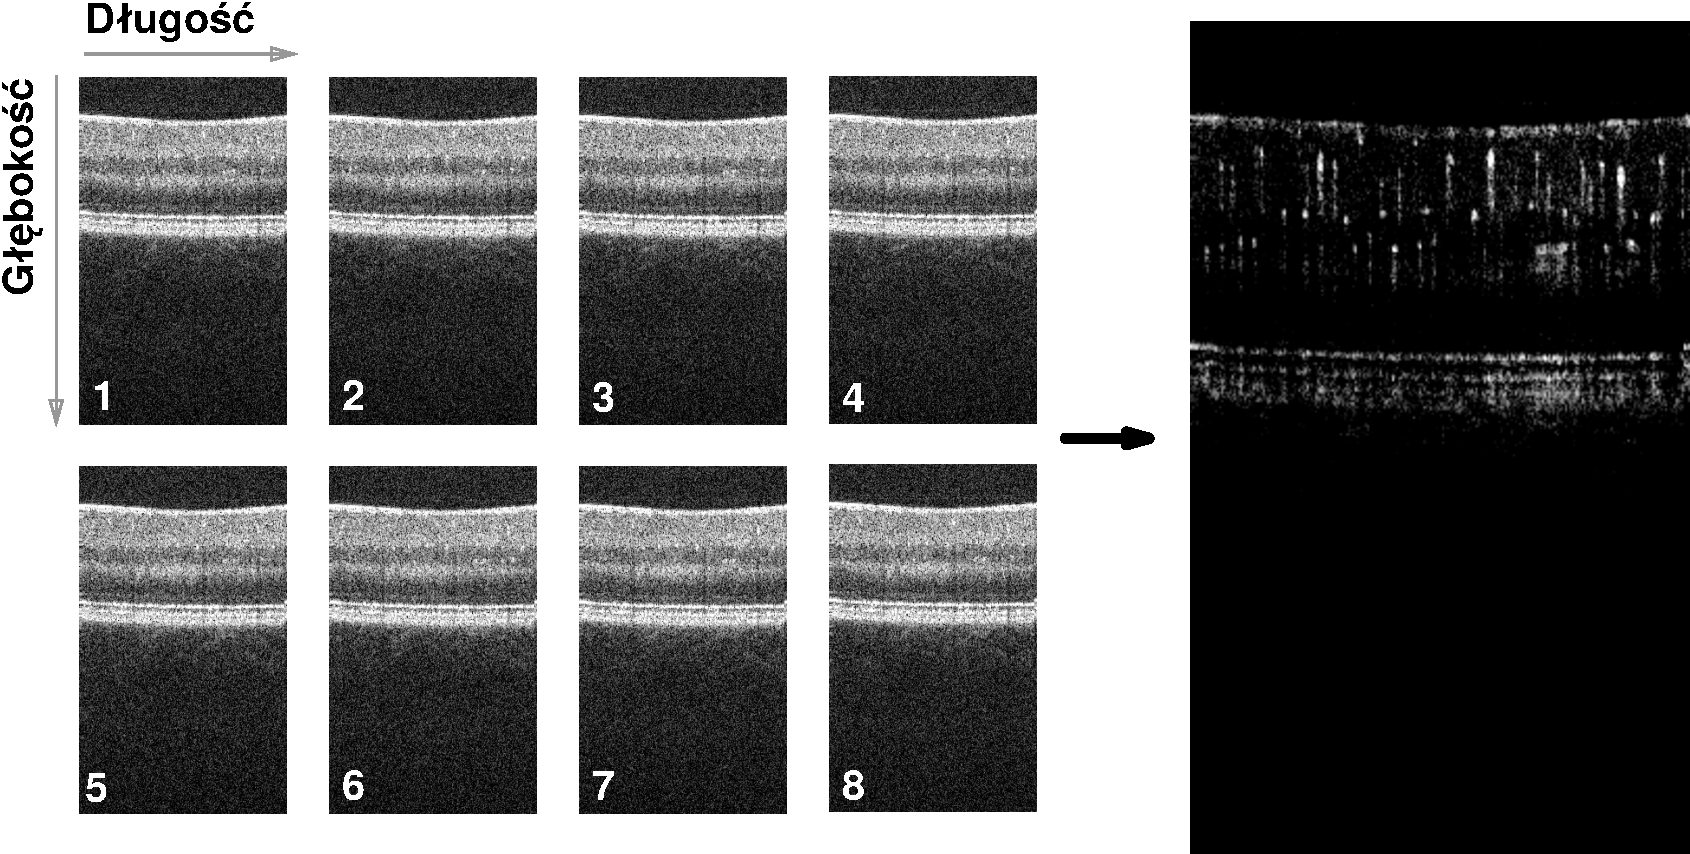
\includegraphics[width=\textwidth]{gfx/speckle_variance}
	\caption{Na lewej stronie przedstawiono osiem sąsiadujących B-skanów na postawie których powstaje jeden obraz przepływowy pokazany na prawej stronie.}
	\label{fig:obrazowanie_oct:speckle_variance}
\end{figure}

Wartości pikseli $V_{jk}$ obrazu przepływowego liczone są na podstawie wartości pikseli $I_{ijk}$ sąsiadujących $N$ B-skanów za pomocą wzoru (na rysunku \ref{fig:obrazowanie_oct:speckle_variance} $N=8$):
\begin{equation}
V_{jk} = \frac{1}{N} \displaystyle\sum_{i=1}^{N}(I_{ijk} - I_{mean})^2
\end{equation}
Gdzie $j$ i $k$ to indeksy boczne i głębokościowe B-skanu (współrzędne pikseli), a $I_{mean}$ to średnia intensywność zbioru tych samych pikseli, dla których liczona jest wariancja.

\begin{figure}[H]
	\centering
	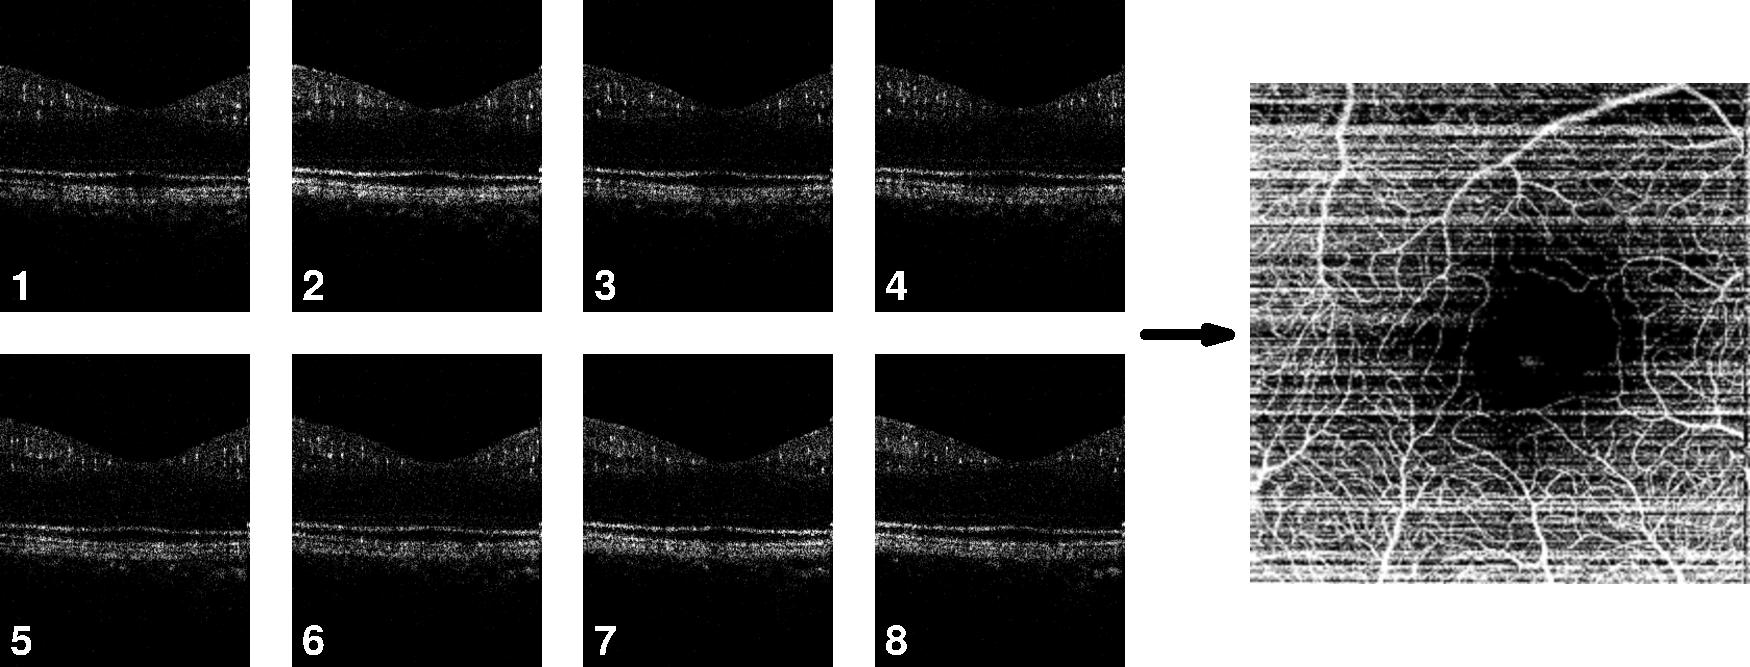
\includegraphics[width=\textwidth]{gfx/en_face_sv}
	\caption{Na lewej stronie znajduje się fragment zbioru sąsiadujących obrazów przepływowych będących częścią na podstawie których powstaje jeden obraz \textit{en face} pokazany na prawej stronie.}
	\label{fig:obrazowanie_oct:en_face_sv}
\end{figure}

Rezultatem połączenia dwuwymiarowych sąsiadujących obrazów przepływowych jest trójwymiarowy obraz przepływowy, który poddaje się projekcji maksymalnego natężenia (ang. \textit{maximum intensity projection, MIP}) polegającej na projekcji woksela o najwyższej intensywności z obrazu 3D na obraz 2D. Po zastosowaniu projekcji maksymalnego natężenia na trójwymiarowym obrazie przepływowym otrzymujemy angiograficzny obraz \textit{en face} naczyń krwionośnych. Rysunek \ref{fig:obrazowanie_oct:en_face_sv} przedstawia część z obrazów przepływowych na podstawie których stworzono jeden obraz \textit{en face}.

% Opisuje zastosowania OCT

\section{Zastosowania OCT}
\label{sec:obrazowanie_oct:zastosowania_oct}

Optyczna tomografia koherencyjna ze względu na swoje właściwości (badanie nieinwazyjne oraz \textit{in vivo}) jest metodą, która ma szerokie zastosowanie w medycynie oraz w innych specjalizacjach.

\subsection{OCT w okulistyce}

Najbardziej popularnym zastosowaniem OCT w medycynie jest badanie oka \cite{Fercher03}. Technika OCT umożliwia przechwycenie trójwymiarowych obrazów części oka takich jak dno, czy warstwy przednie. Dzięki temu jest wykorzystywane do diagnozowania takich chorób jak stwardnienie rozsiane, zwyrodnienie plamki żółtej, czy jaskra.

\subsection{OCT w gastroenterologii i dermatologii}

OCT w porównaniu do innych metod diagnostycznych w medycynie jest techniką nową. Lekarze i naukowcy nieustannie starają się znaleźć nowe zastosowania dla OCT, która jest metodą obiecującą i szybko rozwijającą się. OCT jest potencjalnym kandydatem by w niektórych diagnozach zastąpić konwencjonalną biopsję wymagającą usunięcia kawałka tkanki z organizmu. Przykładowe zastosowania OCT:

\begin{itemize}
\item \textbf{Badanie struktury błon śluzowych i podśluzowych w układzie pokarmowym.} OCT dostarczyło czyste obrazy dostarczające lekarzom dużo diagnostycznej informacji \cite{Rollins:99}.
\item \textbf{Diagnoza raka skóry} (obecnie diagnozowany jest poprzez biopsję). Niestety OCT w obecnym stopniu zaawansowania nie jest w stanie dostarczyć na tyle dokładnych danych by stać się jedyną metodą diagnozy.
\item \textbf{Diagnoza zapalnych chorób skóry} \cite{Welzel01}.
\end{itemize}

\subsection{OCT w przemyśle}

OCT wykorzystywane jest również w przemyśle. Umożliwia badanie np. grubości materiałów \cite{walecki2006determining}, czy badanie grubości warstwy pancerza tabletek podczas ich produkcji w przemyśle farmaceutycznym \cite{markl2014device}.

% !TEX root = ../thesis-example.tex
%
\chapter{Algorytmy korejestracji przestrzennej obrazów OCT}
\label{sec:algorytmy_korejestracji}

\textbf{Mozaiką} nazywa się obraz, który powstaje poprzez połączenie grupy obrazów zwanych kafelkami na podstawie ich wzajemnych relacji. Znanym oraz popularnym przykładem łączenia obrazów w jeden większy jest funkcja panoramy w telefonach komórkowych, czy aparatach fotograficznych. Od strony użytkownika proces tworzenia panoramy polega na powolnym przesuwaniu telefonem po linii poziomej do momentu aż żądany krajobraz zostanie uchwycony. Od strony urządzenia proces polega na wykonywaniu serii zdjęć oraz następnie łączenie nachodzących klatek w jeden obraz. Rezultatem jest jednolita panorama, która składa się z grupy mniejszych węższych zdjęć.

Celem niniejszej pracy jest stworzenie mozaiki OCT (przykład na rysunku \ref{fig:algorytmy_korejestracji:mosaic}), która powstaje z połączenia mniejszych nachodzących na siebie nawzajem angiograficznych obrazów OCT (przykład obrazu angiograficznego OCT znajduje się z prawej strony na rysunku \ref{fig:obrazowanie_oct:bscan_vessels}).

\begin{figure}[H]
  \centering
  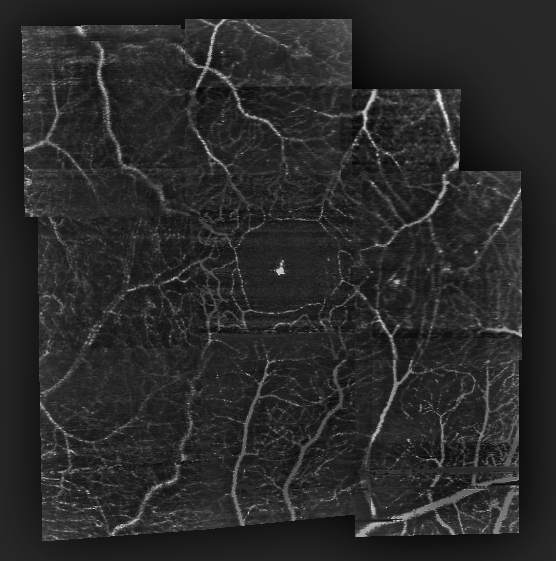
\includegraphics[width=10cm]{gfx/mosaic}
  \caption{Mozaika OCT stworzona z połączenia angiograficznych obrazów OCT.}
  \label{fig:algorytmy_korejestracji:mosaic}
\end{figure}

Proces automatycznego stworzenia mozaiki takiej jak na rysunku \ref{fig:algorytmy_korejestracji:mosaic} jest zadaniem nietrywialnym i wymaga dokładnej analizy wiedzy dziedzinowej oraz precyzyjnego wyboru metod. Pierwszym krokiem jest wybór modelu deformacji kafelków (sekcja \ref{sec:algorytmy_korejestracji:model_deformacji}), następnym etapem, który jest jednocześnie najbardziej wymagającym jest wybór metody wzajemnej korejestracji kafelków (sekcja \ref{sec:algorytmy_korejestracji:korejestracja_kafelow}). Posiadając zdefiniowane wzajemne relacje kafelków oraz ich docelowe położenie w finalnej mozaice należy wykonać proces łączenia kafelków (sekcja \ref{sec:algorytmy_korejestracji:laczenie_kafelkow}). W każdej z tych sekcji została wyjaśniona idea metody w kontekście stworzenia mozaiki OCT, natomiast szczegółowy opis zaimplementowanych metod znajduje się w rozdziale \ref{sec:proponowane_algorytmy}.

\section{Model deformacji kafelków}
\label{sec:algorytmy_korejestracji:model_deformacji}

Model deformacji kafelków określa dozwolone przekształcenia geometryczne, które odwzorują piksele kafelka do pikseli kafelka w finalnej mozaice. Ze względu na to, że angiograficzne obrazy OCT znajdują się na jednej płaszczyźnie możliwy zbiór modeli deformacji ogranicza nam się do transformacji dwuwymiarowych, które zostały zobrazowane na rysunku \ref{fig:algorytmy_korejestracji:trans}.

\begin{figure}[H]
  \centering
  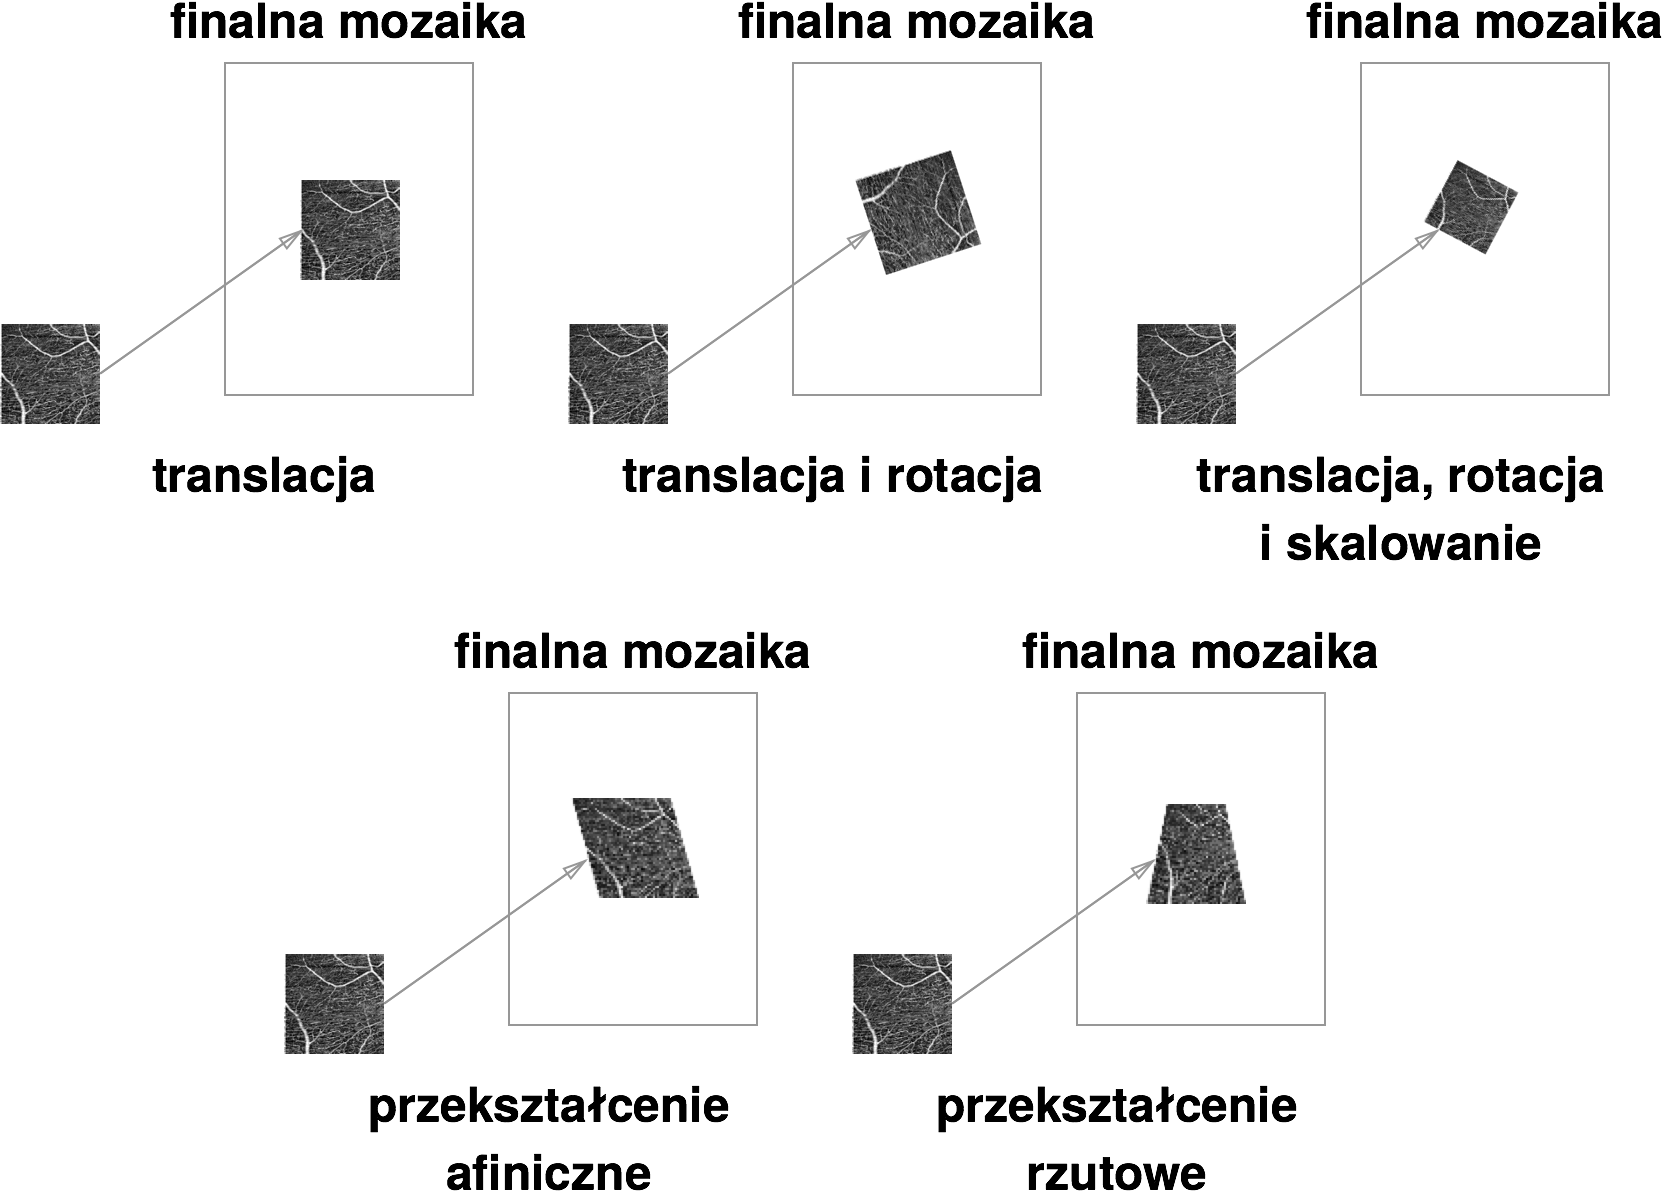
\includegraphics[width=\textwidth]{gfx/trans}
  \caption{Zbiór transformacji dwuwymiarowych dla przykładowego angiograficznego obrazu OCT.}
  \label{fig:algorytmy_korejestracji:trans}
\end{figure}

Idealnie OCT powinno tworzyć angiograficzne obrazy, które są względem siebie tylko przesunięte, natomiast w rzeczywistości pojawiają się zniekształcenia wynikające z niedokładności urządzenia oraz ruchu oka pacjenta, przez co niektóre kafelki są nieznacznie obrócone względem siebie. Z tego względu wybranym modelem deformacji kafelków został \textbf{model transformacji ciała sztywnego}, czyli połączenie translacji i rotacji.

\subsection{Matematyczny zapis modelu transformacji ciała sztywnego}

Współrzędne piksela w kafelku możemy określić jako trójelementowy wektor $\widetilde{x}=(x, y, 1)$, gdzie $x$ i $y$ to współrzędne piksela w układzie współrzędnych kafelka. Tak zdefiniowany piksel poddaje się transformacji by uzyskać współrzędne tego piksela $\hat{x}=(x', y')$ w układzie współrzędnych finalnej mozaiki. W sekcji \ref{sec:algorytmy_korejestracji:model_deformacji} została wybrana transformacja ciała sztywnego, który zakłada tylko translację oraz rotację i może być zapisana jako:

\begin{equation}
\hat{x}=\begin{bmatrix}R&t\end{bmatrix}\widetilde{x}
\label{eq:transformation}
\end{equation}

gdzie:

\begin{align}
R &= \begin{bmatrix}cos(\theta)&-sin(\theta)\\sin(\theta)&cos(\theta)\end{bmatrix} &&\text{i} & t &= \begin{bmatrix}t_{x}\\t_{y}\end{bmatrix}
\label{eq:rotation_and_translation}
\end{align}

W równaniu \ref{eq:rotation_and_translation} $\theta$ to kąt obrotu (rotacja) względem początku układu współrzędnych, a $t_{x}$ i $t_{y}$ to odpowiednio przesunięcia względem osi x i osi y. Parametry $\theta$, $t_{x}$ i $t_{y}$ są niewiadomymi równania \ref{eq:transformation}, których obliczenie jest tematem sekcji \ref{sec:algorytmy_korejestracji:korejestracja_kafelow}.

\section{Korejestracja kafelków}
\label{sec:algorytmy_korejestracji:korejestracja_kafelow}

Po wyborze modelu deformacji kafelków można przejść do wyboru metody, która będzie określać jego parametry (w przypadku niniejszej pracy są to parametry przesunięcia i obrotu). Metoda ta powinna zwrócić takie wartości by kafelek znalazł się w odpowiednim miejscu w finalnej mozaice z możliwie najmniejszym błędem. By rozwiązać ten problem najpierw trzeba poznać położenie kafelków względem siebie oraz ustalić kafelek referencyjny. Rysunek \ref{fig:algorytmy_korejestracji:reference_tile} przedstawia przykładowe rozmieszczenie kafelków. Kafelek referencyjny oznaczony poprzez przerywane linie jest przesuwany do finalnej mozaiki, natomiast żeby odpowiednio umieścić kafelki (2) i (3) trzeba najpierw znać dopasowanie kafelków (2) i (3) do kafelka referencyjnego (1). W przykładzie na rysunku \ref{fig:algorytmy_korejestracji:reference_tile} zostało założone, że kafelki (2) i (3) mogą być dopasowane do kafelka (1). Informacja na temat tego, które kafelki należy dopasować do których kafelek wynika z wiedzy dziedzinowej i opisane jest to w sekcji \ref{sec:proponowane_algorytmy:wiedza_dziedzinowa}.

\begin{figure}[H]
  \centering
  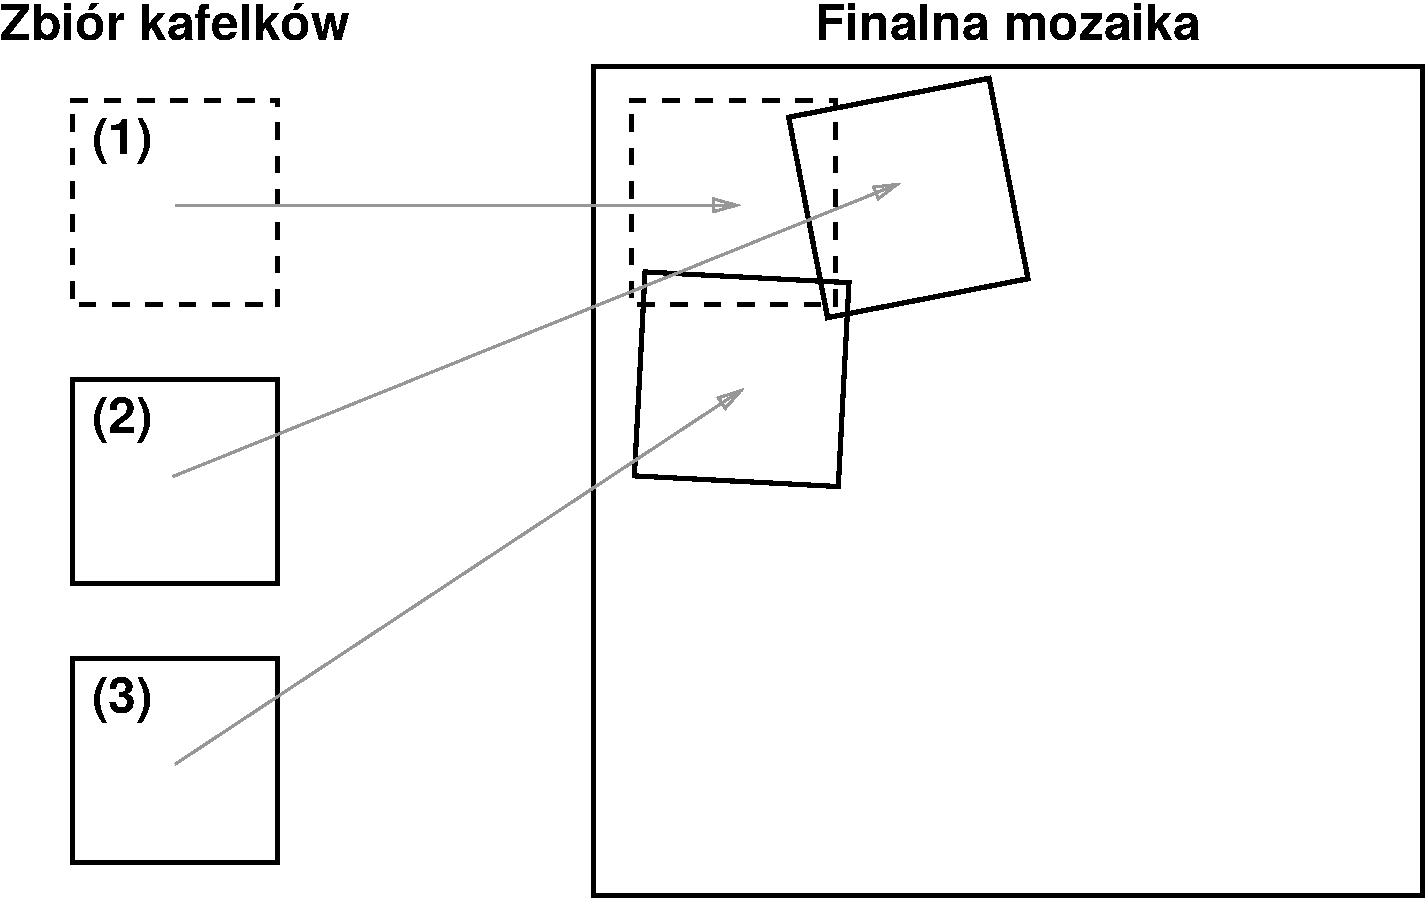
\includegraphics[width=\textwidth]{gfx/reference_tile}
  \caption{Przykładowe rozmieszczenie kafelków na finalnej mozaice. Kafelek referencyjny został wyróżniony przerywaną linią.}
  \label{fig:algorytmy_korejestracji:reference_tile}
\end{figure}

Dopasowanie dwóch kafelków do siebie nazywa się również ich korejestracją, czyli przeniesieniem dwóch kafelków do wspólnego układu współrzędnych w taki sposób by były względem siebie dopasowane. Prosty przykład korejestracji przedstawiony jest na rysunku \ref{fig:algorytmy_korejestracji:align}, gdzie dwie kafelki mają wspólny obszar nałożenia.

\begin{figure}[H]
  \centering
  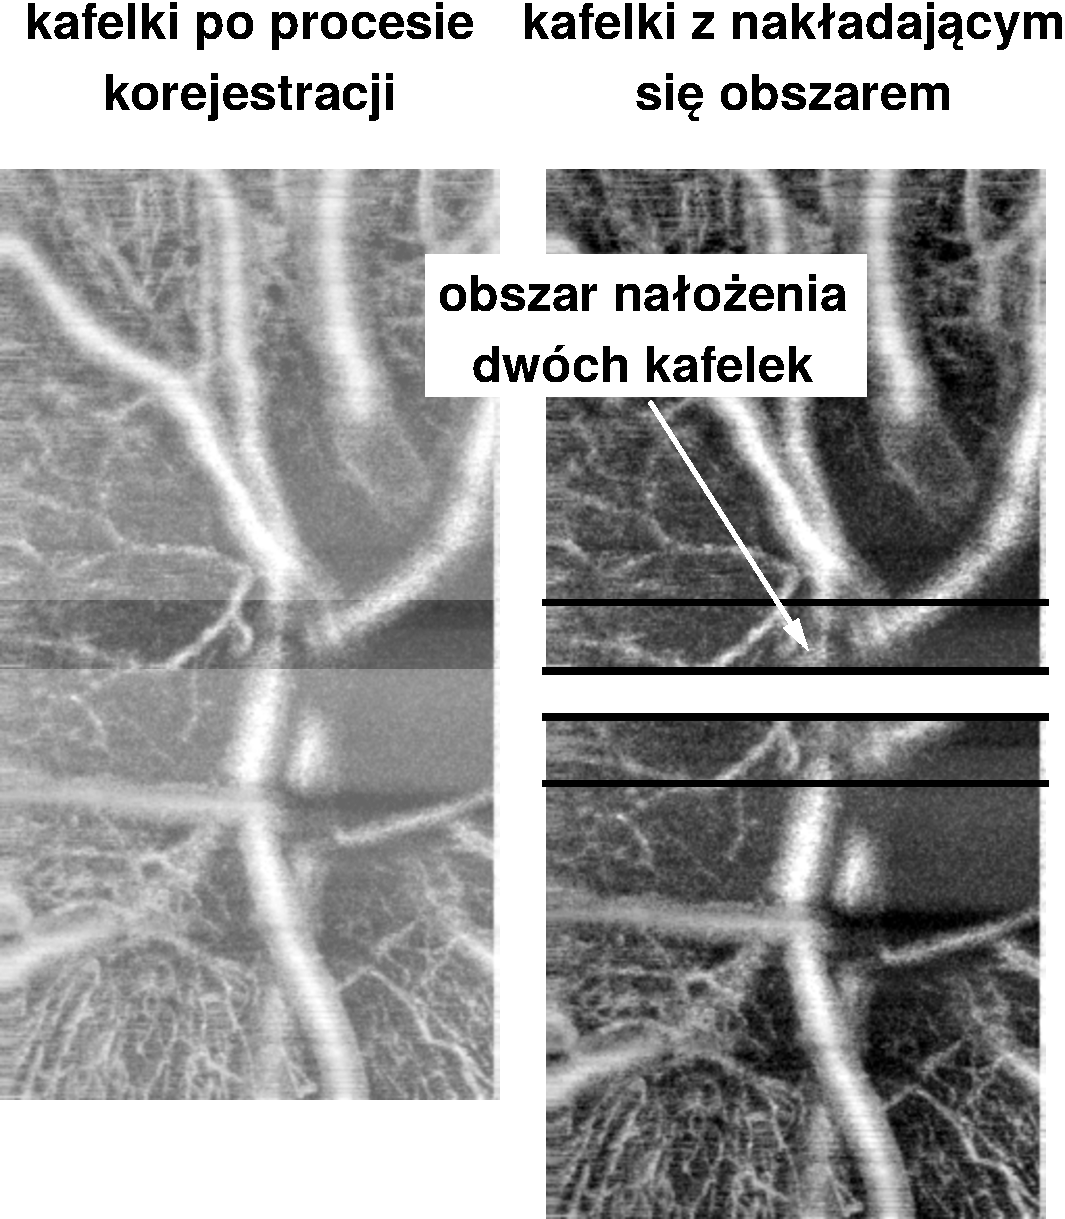
\includegraphics[width=7cm]{gfx/align}
  \caption{Przykładowa korejestracja dwóch kafelków ze wspólnym obszarem nałożenia.}
  \label{fig:algorytmy_korejestracji:align}
\end{figure}

Dopasowanie kafelków z rysunku \ref{fig:algorytmy_korejestracji:align} jest przykładem bardzo prostym, ponieważ wymaga tylko translacji jednego kafelka względem drugiego. W rzeczywistości pomiary OCT nie są tak dokładne przez co prosta translacja wzdłuż jednej z osi nie wystarcza i wymagane jest automatyczne wyznaczenie parametrów translacji i rotacji, które może być wykonane na wiele sposobów. Dwie najpopularniejsze metody to:

\begin{enumerate}
\item \textbf{Korejestracja na podstawie wartości pikseli} (sekcja \ref{sec:algorytmy_korejestracji:korejestracja_na_podstawie_wartosci}) - Metoda przesuwająca jeden obraz względem drugiego i następnie oceniająca jak nałożone piksele obrazów pasują do siebie na podstawie ich wartości.
\item \textbf{Korejestracja na podstawie cech} (sekcja \ref{sec:algorytmy_korejestracji:korejestracja_na_podstawie_cech}) - Metoda wyodrębniająca charakterystyczne cechy z każdego obrazu i następnie dopasowująca te cechy by osiągnąć globalną spójność. Dopasowania są później użyte przez algorytm do wyznaczenia macierzy transformacji pomiędzy obrazami.
\end{enumerate}

\subsection{Korejestracja na podstawie wartości pikseli (bezpośrednie)}
\label{sec:algorytmy_korejestracji:korejestracja_na_podstawie_wartosci}

\subsection{Korejestracja na podstawie cech}
\label{sec:algorytmy_korejestracji:korejestracja_na_podstawie_cech}

\section{Łączenie kafelków}
\label{sec:algorytmy_korejestracji:laczenie_kafelkow}





















% !TEX root = ../thesis-example.tex
%
\chapter{Proponowane algorytmy}
\label{sec:proponowane_algorytmy}

\section{Wiedza dziedzinowa}
\label{sec:proponowane_algorytmy:wiedza_dziedzinowa}

\section{Wykrywanie naczyń krwionośnych za pomocą Depth First Search}
\label{sec:proponowane_algorytmy:depth_first_search}

\section{Ekstrakcja cech za pomocą SIFT}
\label{sec:proponowane_algorytmy:sift}

\section{RANSAC}
\label{sec:proponowane_algorytmy:ransac}

\section{Filtrowanie dopasowań}
\label{sec:proponowane_algorytmy:filtrowanie}

\section{Estymacja macierzy transformacji}
\label{sec:proponowane_algorytmy:estymacja}

\section{Łączenie kafelków}
\label{sec:proponowane_algorytmy:laczenie_kafelkow}
% !TEX root = ../thesis.tex
%
\chapter{Wyniki eksperymentów obliczeniowych}
\label{sec:wyniki_eksperymentow}

% !TEX root = ../thesis.tex
%
\chapter{Podsumowanie i wnioski końcowe}
\label{sec:podsumowanie_i_wnioski}

% \section{System Section 1}
% \label{sec:obrazowanie_oct:sec1}
\cleardoublepage

% --------------------------
% Back matter
% --------------------------
{%
\setstretch{1.1}
\renewcommand{\bibfont}{\normalfont\small}
\setlength{\biblabelsep}{0pt}
\setlength{\bibitemsep}{0.5\baselineskip plus 0.5\baselineskip}
\printbibliography[nottype=online]
\printbibliography[heading=subbibliography,title={Strony internetowe},type=online,prefixnumbers={@}]
}
\cleardoublepage

\listoffigures
\cleardoublepage

\listoftables
\cleardoublepage

\newpage
\mbox{}

% **************************************************
% End of Document CONTENT
% **************************************************
\end{document}
